%% SmartFitao Computer Vision (Camera Work) — CAS-style overview
\documentclass[a4paper,fleqn]{cas-sc}

\usepackage[authoryear,longnamesfirst]{natbib}
\usepackage{graphicx}
\usepackage{booktabs}
\usepackage{array}
\usepackage{tabularx}
\usepackage{amsmath}
\usepackage{setspace}
\usepackage{xcolor}
\usepackage{colortbl}
\usepackage{tikz}
\usetikzlibrary{shapes,arrows.meta,positioning,fit,backgrounds}
\usepackage[colorlinks=true,linkcolor=blue,urlcolor=blue,citecolor=blue]{hyperref}

\setstretch{1.05}
\setlength{\parskip}{0.4em}
\renewcommand{\arraystretch}{1.5}

\definecolor{tblhead}{RGB}{230,240,255}
\definecolor{tblrowA}{RGB}{255,255,255}
\definecolor{tblrowB}{RGB}{245,248,252}
\definecolor{flowblue}{RGB}{220,235,255}
\definecolor{flowgreen}{RGB}{220,245,220}
\definecolor{floworange}{RGB}{255,235,210}

\newcommand{\tblheadrow}{\rowcolor{tblhead}}

\begin{document}
\let\WriteBookmarks\relax

\shorttitle{SmartFitao Live Pose Capture}
\shortauthors{A. Farooq et al.}

\title[mode=title]{SmartFitao Live Pose Capture: MediaPipe BlazePose Landmarks for Body-Measurement Pipeline Entry}

\tnotetext[1]{Module: \texttt{Computer Vision (Camera Work)}. Default service port: 5000. Export schema: \texttt{Smart\_Fitao\_LivePose}.}

\author[1]{Asif Farooq}[%
  type=editor,
  auid=001,
  role=Researcher]
\cormark[1]
\ead{asif.farooq@ucp.edu.pk}
\credit{Conceptualization, Methodology, Supervision}

\author[2]{Nauman Irshad Ali Shah}
\ead{L1F22BSCS0122@ucp.edu.pk}
\credit{Software, Integration, Flutter bridge}

\author[3]{Umer Amir}
\credit{Investigation, Validation}

\author[4]{Ali Ahmad}
\credit{Software, UI implementation}

\author[5]{Abdul Rehman}
\credit{Resources, Writing - review \& editing}

\affiliation[1]{organization={Department of Computer Science, University of Central Punjab},
  addressline={Khayaban-e-Jinnah Road},
  city={Lahore},
  postcode={54000},
  country={Pakistan}}

\cortext[cor1]{Corresponding author}

\begin{abstract}
This document describes the Computer Vision (Camera Work) module of the SmartFitao FYP platform. The system guides a user into a full-body stand zone, detects \textbf{33 body keypoints} in real time using Google MediaPipe \textbf{BlazePose}, validates posture and A-pose heuristics, and captures a JPEG only when quality gates pass. Inference runs in the browser (live camera) and is re-verified on the server (\texttt{POST /analyze}). Landmarks and confidence scores are exported under the \texttt{Smart\_Fitao\_LivePose} JSON schema for downstream 2D try-on and 3D studio flows. No custom neural training is performed; all pose estimation uses pretrained MediaPipe Pose (\texttt{model\_complexity=1}).
\end{abstract}

\begin{keywords}
MediaPipe \sep BlazePose \sep body landmarks \sep Flask \sep OpenCV \sep SmartFitao \sep FYP
\end{keywords}

\maketitle

\section{INTRODUCTION}

The Camera Work module is the \textbf{entry point} for body-aware features in SmartFitao: live pose validation before photos are saved for AI cloth size prediction, 2D virtual try-on (\texttt{id-2d-try-on}), or 3D avatar studio (port 5001). Unlike a generic webcam app, it enforces:

\begin{itemize}
  \item Full-body visibility inside a stand zone
  \item Minimum landmark visibility (default $\geq 30/33$ points at visibility $\geq 0.65$)
  \item Posture checks (shoulders above hips, ankles below hips)
  \item Optional A-pose arm-angle validation
\end{itemize}

The module does \textbf{not} train custom models. It wraps MediaPipe Pose with application-specific quality scoring and Flutter WebView integration.

\section{TECHNOLOGY STACK}

\begin{table}[h]
\centering
\caption{Software stack by layer}
\label{tab:stack}
\begin{tabularx}{\linewidth}{@{}lX@{}}
\tblheadrow
\textbf{Layer} & \textbf{Technologies} \\
\midrule
Server & Python 3, \textbf{Flask 3.0}, Werkzeug, optional Gunicorn \\
Computer vision & \textbf{OpenCV} (\texttt{opencv-python-headless}), \textbf{MediaPipe}, NumPy \\
Browser client & HTML5 Canvas, \textbf{MediaPipe JS} (Pose, Camera utils, drawing utils) \\
Mobile bridge & Flutter \texttt{webview\_flutter}, \texttt{SmartFitaoCv} JS channel \\
Utilities & \texttt{qrcode[pil]}, \texttt{pyopenssl} (optional HTTPS) \\
Storage & Local folder \texttt{images/} (JPEG captures) \\
\end{tabularx}
\end{table}

\textbf{Default ports:} camera app \texttt{5000}; 3D studio \texttt{5001} (separate service).

\section{POSE MODEL}

\begin{table}[h]
\centering
\caption{Models used (no custom training)}
\label{tab:models}
\begin{tabularx}{\linewidth}{@{}llX@{}}
\tblheadrow
\textbf{Stage} & \textbf{Model} & \textbf{Configuration} \\
\midrule
Live camera (browser) & MediaPipe \textbf{BlazePose} & \texttt{modelComplexity: 1}, \texttt{minDetectionConfidence: 0.6}, \texttt{minTrackingConfidence: 0.6} \\
Still image (server) & MediaPipe \textbf{Pose} (Python) & \texttt{static\_image\_mode=True}, \texttt{model\_complexity=1}, \texttt{min\_detection\_confidence=0.5} \\
Fallback & Mock random landmarks & Used if MediaPipe unavailable (e.g.\ Python 3.13) \\
\end{tabularx}
\end{table}

\textbf{Not used:} OpenPose, YOLO, MediaPipe Face Mesh as a separate model, TensorFlow/PyTorch fine-tuning.

\section{LANDMARK DETECTION PIPELINE}

\subsection{Overview}

Figure~\ref{fig:pipeline} summarizes dual inference: real-time browser pose for UX gating, server pose on captured JPEG for persistence and API response.

\begin{figure}[h]
\centering
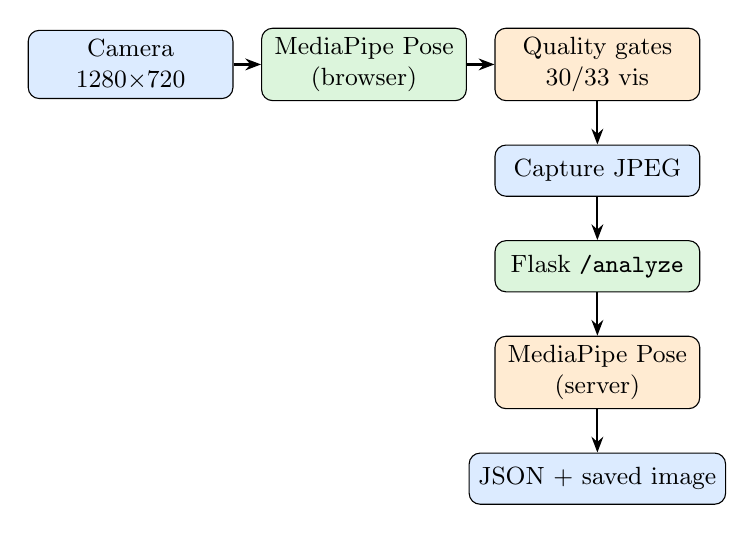
\begin{tikzpicture}[
  node distance=0.55cm and 0.35cm,
  box/.style={draw, rounded corners, minimum width=2.6cm, minimum height=0.65cm, align=center, font=\small},
  arr/.style={-{Stealth[length=2mm]}, thick}
]
  \node[box, fill=flowblue] (cam) {Camera\\1280$\times$720};
  \node[box, fill=flowgreen, right=of cam] (mpjs) {MediaPipe Pose\\(browser)};
  \node[box, fill=floworange, right=of mpjs] (gate) {Quality gates\\30/33 vis};
  \node[box, fill=flowblue, below=of gate] (cap) {Capture JPEG};
  \node[box, fill=flowgreen, below=of cap] (api) {Flask \texttt{/analyze}};
  \node[box, fill=floworange, below=of api] (mppy) {MediaPipe Pose\\(server)};
  \node[box, fill=flowblue, below=of mppy] (json) {JSON + saved image};

  \draw[arr] (cam) -- (mpjs);
  \draw[arr] (mpjs) -- (gate);
  \draw[arr] (gate) -- (cap);
  \draw[arr] (cap) -- (api);
  \draw[arr] (api) -- (mppy);
  \draw[arr] (mppy) -- (json);
\end{tikzpicture}
\caption{End-to-end landmark detection and capture pipeline}
\label{fig:pipeline}
\end{figure}

\subsection{How landmarks are found}

MediaPipe BlazePose outputs \textbf{33 landmarks} per frame in normalized image coordinates:
\begin{equation}
  \mathbf{p}_i = (x_i, y_i, z_i, v_i), \quad i \in \{0,\ldots,32\}
\end{equation}
where $x_i, y_i \in [0,1]$, $z_i$ is depth relative to hip, and $v_i$ is \textbf{visibility} $\in [0,1]$.

Detection steps:
\begin{enumerate}
  \item \textbf{Person detection} --- BlazePose internal detector finds a person bounding region.
  \item \textbf{Pose regression} --- 33 keypoints regressed on the crop (complexity level 1 = balanced speed/accuracy).
  \item \textbf{Tracking} --- consecutive frames reuse prior pose for stability (\texttt{minTrackingConfidence}).
  \item \textbf{Overlay} --- skeleton drawn via \texttt{POSE\_CONNECTIONS}; each dot colored by visibility.
  \item \textbf{Capture gate} --- count landmarks with $v_i \geq 0.65$; require $\geq 30$ of 33 (configurable via \texttt{?min\_landmarks=}).
  \item \textbf{Server verify} --- saved JPEG re-processed; same 33 points serialized to JSON.
\end{enumerate}

\subsection{All 33 landmark names (MediaPipe order)}

\begin{table}[h]
\centering
\caption{Smart\_Fitao\_LivePose keypoints (schema version 1)}
\label{tab:landmarks}
\small
\begin{tabular}{@{}clcl@{}}
\tblheadrow
\textbf{Idx} & \textbf{Name} & \textbf{Idx} & \textbf{Name} \\
\midrule
0 & nose & 17 & left\_pinky \\
1--10 & eyes, ears, mouth & 18--22 & right hand fingers \\
11 & left\_shoulder & 23 & left\_hip \\
12 & right\_shoulder & 24 & right\_hip \\
13--16 & elbows, wrists & 25--32 & knees, ankles, feet \\
\end{tabular}
\end{table}

Full names are fixed in \texttt{\#smart-fitao-pose-spec} embedded in \texttt{templates/index.html}.

\section{FEATURES AND QUALITY METRICS}

\subsection{Per-landmark features}

Each landmark exports: \texttt{id}, \texttt{name}, \texttt{x}, \texttt{y}, \texttt{z}, \texttt{visibility}.

\subsection{Derived quality features}

\begin{table}[h]
\centering
\caption{Human-presence and capture quality metrics}
\label{tab:metrics}
\begin{tabularx}{\linewidth}{@{}lX@{}}
\tblheadrow
\textbf{Feature} & \textbf{Definition} \\
\midrule
\texttt{human\_probability} & $0.25\,\overline{v_{\mathrm{all}}} + 0.45\,\overline{v_{\mathrm{core}}} + 0.30\,(\mathrm{strong\_core}/7)$ \\
\texttt{human\_detected} & \texttt{human\_probability} $\geq 0.42$ and $\geq 4$ core joints with $v \geq 0.4$ \\
Core indices & 0, 11, 12, 23, 24, 27, 28 (nose, shoulders, hips, ankles) \\
Capture threshold & $\geq 30/33$ landmarks with visibility $\geq 0.65$ \\
Posture OK & Core vis $\geq 0.6$, in-frame margins, hips below shoulders \\
A-pose OK & Arm angle heuristics ($\approx$18°--58° from vertical) \\
\end{tabularx}
\end{table}

\subsection{Results returned by \texttt{POST /analyze}}

\begin{table}[h]
\centering
\caption{API response fields (operational metrics, not ML benchmark)}
\label{tab:api}
\begin{tabular}{@{}ll@{}}
\tblheadrow
\textbf{Field} & \textbf{Meaning} \\
\midrule
\texttt{human\_detected} & Boolean body present \\
\texttt{human\_probability} & 0--1 confidence score \\
\texttt{landmarks\_count} & Typically 33 or 0 \\
\texttt{landmarks[]} & Full 33-point list \\
\texttt{saved\_filename} & JPEG under \texttt{images/} \\
\texttt{image\_url} & \texttt{/captured/<filename>} \\
\end{tabular}
\end{table}

\textbf{Note:} There is no held-out test accuracy, mAP, or PCK in this module---only heuristic gates for capture quality.

\section{API AND INTEGRATION}

\begin{table}[h]
\centering
\caption{Flask routes}
\label{tab:routes}
\begin{tabular}{@{}ll@{}}
\tblheadrow
\textbf{Route} & \textbf{Purpose} \\
\midrule
\texttt{GET /} & Pose Auto-Capture SPA \\
\texttt{GET /qr} & QR code for mobile camera URL \\
\texttt{POST /analyze} & Upload image, run pose, save JPEG, return JSON \\
\texttt{GET /captured/<file>} & Serve saved capture \\
\end{tabular}
\end{table}

\textbf{Flutter integration:} embed with \texttt{?flutter\_embed=1}; events via \texttt{postMessage} type \texttt{smartfitao\_cv} (phases: \texttt{live}, \texttt{capture}, \texttt{move\_3d\_avatar}).

\textbf{Downstream:} \texttt{id-2d-try-on} reads user photos from \texttt{Computer Vision (Camera Work)/images}.

\section{LIMITATIONS AND FUTURE WORK}

\begin{itemize}
  \item No custom model training or dataset labeling pipeline in-repo.
  \item Mock fallback when MediaPipe fails---unsuitable for research evaluation.
  \item Anthropometric fields (\texttt{height\_cm}, \texttt{weight\_kg}, \texttt{age}) defined in schema but not yet wired from URL params.
  \item README references \texttt{ImageSaved/}; code uses \texttt{images/}.
\end{itemize}

\section{CONCLUSION}

The Camera Work module provides a production-ready \textbf{live pose capture gate} using pretrained MediaPipe BlazePose (33 landmarks), dual browser/server inference, and SmartFitao-specific quality heuristics. It feeds the broader FYP stack (2D try-on, size prediction, 3D studio) without requiring a separately trained pose model.

\end{document}
